\subsection{Understanding Protection Overhead}
\label{vfree:sec:inefficiencies}
This section builds an in-depth understanding of inefficiencies in existing strict intra-VM IO memory protection mechanisms. We present more results, including those for real-world applications 
  in \S\ref{vfree:sec:eval}.
%We also provide insights into the fundamental reasons behind the observed degradation. 
% Our key findings are:
% \begin{itemize}[leftmargin=*]
% \item State-of-the-art IO memory protection mechanisms introduce significant performance degradation---reducing 
%   the peak throughput by as much as {$\sim$}60-95\% compared to the no protection case. 
%   Using additional cores to run networked applications does not improve throughput; 
%   in fact, we observe a surprising phenomenon: beyond a certain point, assigning more cores to the application can actually result in lower than the peak throughput. 
% % throughput reaches only 145\,Gbps at 12~cores and then \emph{decreases} with additional cores---dropping by 3$\times$ at 24~cores---exhibiting anti-scaling behavior.

% \item The {\it root cause} of low peak throughput is that today each invalidation request (IR)
% %  is serialized across all threads in the VM, 
%   necessitates {\it at least one VM exit}. 
%   This limits the maximum aggregate rate of IRs, 
%   and thus the maximum achievable network throughput, independent of the number of cores running the application. 

% % is not the cost of any single VM~exit, but the \emph{serialization} of all cores' invalidations through a single hardware resource whose access requires a VM~exit.  This serialization caps the system's aggregate invalidation throughput independent of core count.
% \item The {\it root cause} for the surprising phenomenon is more subtle. Virtualization introduces an intricate feedback loop between lock contention 
%   and hypervisor scheduling: 
%   when vCPUs contend for invalidation, those that fail to aquire the lock are descheduled by the hypervisor. 
% Waking these vCPUs requires hypercalls and inter-processor interrupts (IPIs) that further trigger 
%   VM~exits, inflating lock acquisition time and causing 
%   even more vCPUs to be descheduled. 
%   Such a feedback loop causes performance to degrade beyond VM-exit overhead
%   %  beyond the serialization-imposed throughput limit
%   as the number of cores increase.
% \end{itemize}

\para{Measurement Setup.}
% \schaic{All comments resolved. @Rachit please check.}
We use two servers directly connected to each other via $400$Gbps Nvidia ConnectX-7 NICs to ensure performance bottlenecks not in the 
  network. 
The servers use Emerald Rapids processor architecture that supports nested translation,
  with Intel Xeon Platinum 8592V CPUs and Intel Xeon Gold 6538Y+ CPUs respectively. 
The former hosts our VMs, 
  and the latter acts as client to send or receive traffic to the VM. 
  % a passive server engaged in Rx or Tx traffic 
  % \rachit{we have to be careful: each server does both Rx and Tx---right?}.  
% Each server has an Nvidia ConnectX-7 NIC; the two NICs connected to Ethernet with 400Gbps access link bandwidth.
% The host server is a 4-socket server; each socket has
%   32 physical cores, 252GB of memory and 150GB/s of memory bandwidth.
  % per-socket. 
The host server, guest VM, and client machines run with Ubuntu 22.04 and Linux v6.12.9. 
% \saksham{KVM/QEMU versions?} 
The VMs are hosted by QEMU v10.0 with nested translation~\cite{yiliu1765qemu}.
% \saksham{Static pinning of vCPUs to physical cores to avoid interference.} 
We place the VMs on the NIC-local NUMA node.
Every vCPU of the VM is pinned to a separate physical core on the host to avoid interference. See \S\ref{vfree:sec:eval} for more details.
  % We disable hyperthreading, CPU frequency scaling (we fix cores at their base frequency), and NUMA balancing for stable performance. 
% We built a ebpf-based tool to measure the performance of guest and host OS.
% \saksham{if we get time, we should add error bars with stddev}.
% \schaic{We already have errors bars in the latest version @Saksham.}

We use Iperf3~\cite{iperf3} to generate network traffic with $4$K MTU size, and measure throughput.
% We measure CPU utilization with sar~\cite{sar}.
% We use eBPF probes to record the execution time and invocation counts of relevant kernel functions.
% We measure VM exit counts, reasons, and time with perf~\cite{perf}.
% We enabled TCP Segmentation Offload (TSO), Generic Receive Offload (GRO), and adaptive Receive Flow Steering (aRFS) 
% to reflect high-performance networks. 
We run each experiment five times, and present the average results and standard deviation. We use two setups to isolate the impact of IO memory protection on Rx and Tx datapaths. In the {\bf Rx-server} setup, the client sends large payloads to the VM; the VM receives these payloads and transmits TCP ACKs back to the client. In the {\bf Tx-server} setup, the VM sends large payloads to the client and receives TCP ACKs from the client.




% We run the VM as receiver (Rx) 
%   and trasmitter (Tx) 
%   of network traffic, respectively, in two sets of experiments; this helps us isolate the impact of I/O memory protection on each setup. \rachit{this continues to be very confusing---saying that VM is the receiver of network traffic is incorrect since it also does Tx. We should precisely define what these two setups are: Rx receives large payloads and transmits ACKs; Tx transmits large payloads and receives ACKs;}
% Tx and Rx cases separately to isolate the impact of I/O memory protection on each datapath
%   (full-system results in \S\ref{vfree:sec:eval}). 
  % \rachit{readers may find this confusing---each server does both Rx and Tx.}
% later in eval section we run an end-to-end scenario where both kinds of traffic are running concurrently.
% \schai{: receive (Figure~\ref{vfree:fig:motivation-rx}) and transmit (Figure~\ref{vfree:fig:motivation-tx}).
% \noindent
% We increase the number of flows (each pinned to a core in the VM)
%   and compare throughput when running with
%   (1) vIOMMU off and (2) vIOMMU with strict memory protection (using nested translation).
% This section presents minimalist results to build an in-depth understanding of inefficiencies in strict intra-guest IO memory protection;  
  

% \begin{figure}
% 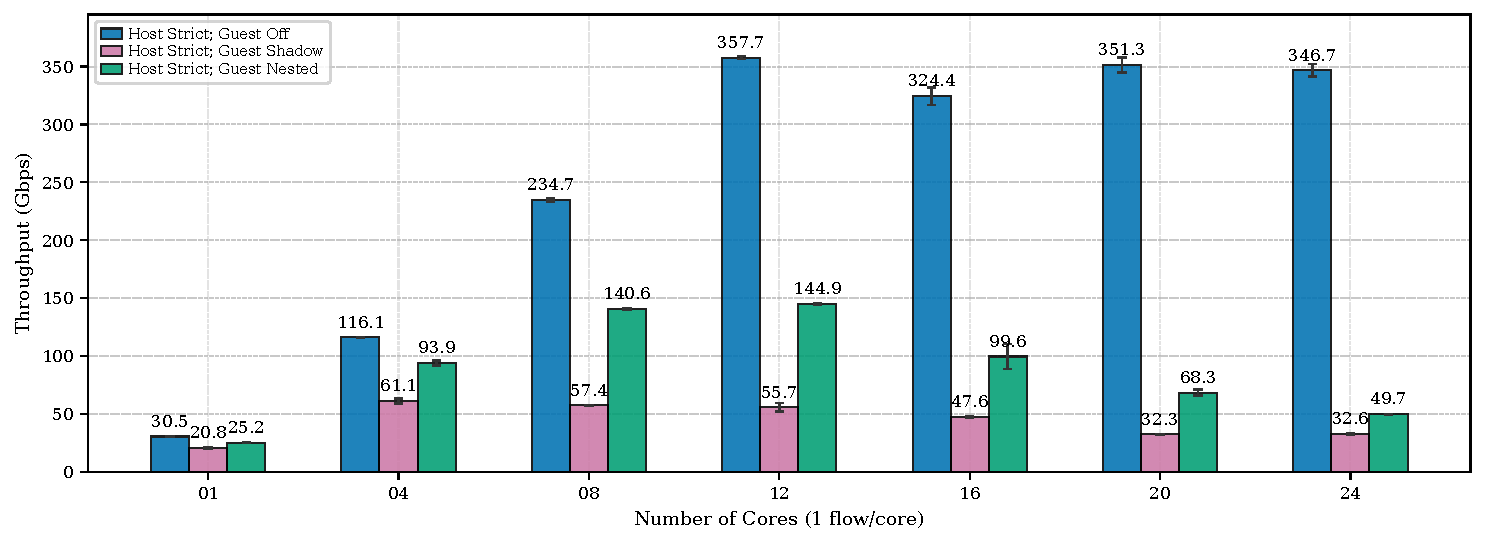
\includegraphics[width=\columnwidth]{figures/baseline-iperf-tput.pdf}
% \Description{Throughput vs Number of Cores Viommu off, Shadow and Nested}
% \caption{Throughput vs Number of Cores Viommu off, Shadow and Nested \saksham{I think we should get rid of shadow results?}}
% \label{vfree:fig:baseline-iperf}
% \end{figure}

\begin{figure}[H]
    \centering
    \begin{subfigure}[b]{\columnwidth}
        \centering
        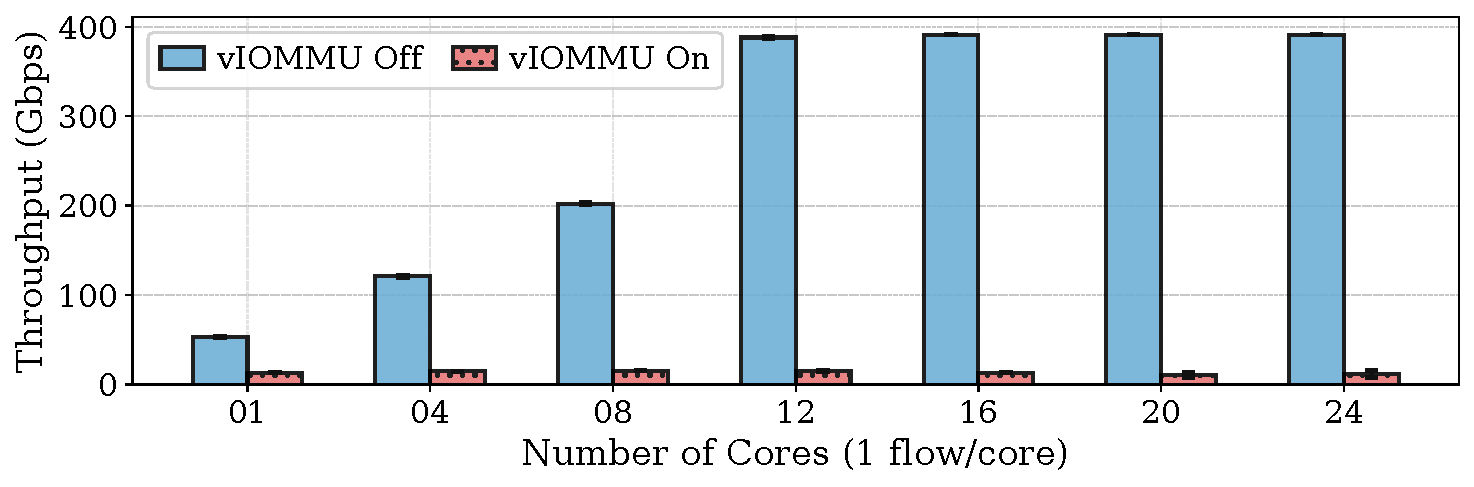
\includegraphics[width=\textwidth]{figures/motivation_tx_varying_cores-tput.pdf}
        \caption{Tx-server (VM running as a transmitter)}
        \label{vfree:fig:motivation-tx}
    \end{subfigure}
    \begin{subfigure}[b]{\columnwidth}
        \centering
        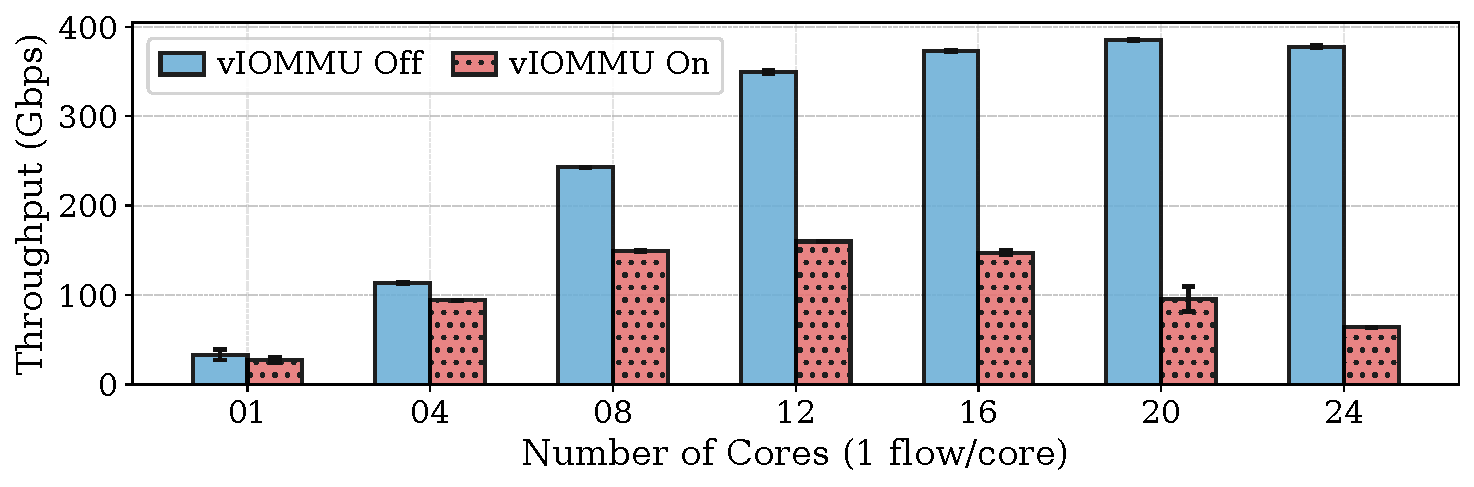
\includegraphics[width=\textwidth]{figures/motivation_rx-tput.pdf}
        % \caption{Rx throughput}
        \caption{Rx-server (VM running as a receiver)}
        \label{vfree:fig:motivation-rx}
    \end{subfigure}
    \caption{\small {\bf State-of-the-art IO memory protection mechanisms suffer from significant performance degradation compared to the unprotected mode,
    and exhibit anti-scaling behavior with increasing cores.} Performance degradation is much more profound on the Tx-server setup.}
    \label{vfree:fig:baseline-iperf}
\end{figure}


\paragraphb{[Figure~\ref{vfree:fig:baseline-iperf}] Performance degradation with IO memory protection in VMs}
% Figure~\ref{vfree:fig:motivation} compares network throughput with increasing number of cores\saksham{should we use vCPUs, or cores in our discussion?} for three configurations: (1) vIOMMU disabled, (2) \sout{vIOMMU strict mode with shadow page tables,} and (3) vIOMMU enabled with strict memory protection and nested translation.
% Figure~\ref{vfree:fig:motivation-rx} and \ref{vfree:fig:motivation-tx} compare network throughput with increasing number of flows (each flow pinned to a core in the VM)
%   for two configurations: (1) vIOMMU disabled and (2) vIOMMU enabled with strict memory protection and nested translation.
Figure~\ref{vfree:fig:motivation-tx} shows throughput for the Tx-server.
Without IO memory protection, $12$ cores are sufficient to saturate the network bandwidth; thus, the achievable throughput increases until $12$ cores and plateaus thereafter.
With IO memory protection enabled, the maximum achievable throughput, 
  irrespective of number of cores used, 
  is ${\sim}$15\,Gbps---a ${\sim}$95+\% degradation 
  compared to no protection.

Figure~\ref{vfree:fig:motivation-rx} shows throughput for the Rx-server.
% With vIOMMU off, the throughput can be as high as ${\sim} 385$Gbps.
%; 12~cores is the minimum to saturate the link, 
 % where Rx throughput reaches 350Gbps .
% \rachit{is 357 the best achievable for a 400gbps link? whats the pcie bandwidth?}
% \sout{Enabling strict mode with shadow page tables---where \emph{both} map and unmap operations require VM~exits---reduces 
  % throughput to 55\,Gbps at 12~cores. }
% \sout{Switching to nested translation, which eliminates VM~exits on the map path, 
%   improves throughput to 145\,Gbps at 12~cores.  
% While nested translation recovers 90\,Gbps compared to shadow mode, 
%   a 60\% gap relative to the unprotected baseline remains.} 
Enabling IO memory protection again results in significant degradation in throughput: we observe a peak throughput of $160$Gbps with $12$ cores---{$\sim$}54\% degradation compared to the no protection case. 
Upon increasing the number of cores beyond 12, the throughput, rather surprisingly, 
  starts to drop; we observed a maximum degradation of up to $\sim$83\% when using 24 cores. 
Compared with the Tx-server case, the relatively higher Rx-server throughput is due to the page pool optimization that reduces map/unmap operations (\S\ref{vfree:sec:background-datapath}); and TCP ACK coalescing, which increases the number of pages 
  per \CodeIn{unmap} (by as much as ${\sim}15\times$).


\if 0
\schai{
We also compare the throughput under the same setup between vIOMMU running on traditional shadow page tables 
  and on nested translation.
We find that the nested translation configuration achieves strictly higher throughput than shadow page tables,
  by 1.2$\times$ to 2.6$\times$ across core counts (\textit{e.g.}, 144.9 vs.\ 55.7\,Gbps at 12~cores).
The difference comes from the fact that with shadow page tables, both map and unmap operations require VM~exits, 
  while with nested translation, only unmap operations require VM~exits.}
\fi

\paragraphb{[Figure~\ref{vfree:fig:lock-contention}] Root cause of performance degradation with IO memory protection: 
  at least one VM exit per unmap/invalidation}
IO memory protection introduces two extra operations on the datapath: \CodeIn{map()} and \CodeIn{unmap()}. 
With nested translation,
\CodeIn{unmap} is far more costly than \CodeIn{map}: 
  besides updating IOPTs, \CodeIn{unmap} also performs IOMMU cache invalidations which 
  require VM exits (\S\ref{vfree:sec:background-datapath}).
We observe that overheads of unmap operations
  are the primary contributor to the performance degradation due to IO memory protection.
  % \footnote{In vanilla Linux,
  %   the overhead of \texttt{\footnotesize unmap} further slows down \CodeIn{map}
  %   as the \texttt{\footnotesize map} implementation tries to acquire 
  %   the \texttt{\footnotesize cache\_lock} for IR processing which is only needed for shadow IOPT, not nested 
  %   translation. Unfortunately, the check is done inside \texttt{\footnotesize cache\_lock}.
  %   We optimized the behavior in \S\ref{vfree:sec:impl}. \rachit{I suggest removing this footnote}}
  % % of the above t degradation 
  % compared to vIOMMU off.

% Our kernel profiling shows that the average \CodeIn{unmap} latency 
%  is orders of magnitude higher than \CodeIn{map}'s\saksham{Verify this} 
% \rachit{precision will be helpful here---present exact numbers}. 
% So, we focus on the \CodeIn{unmap} to understand the root causes of observed performance trends. 

We observe that processing IRs within the \CodeIn{unmap} operation accounts for over {$95\%$} of the total \CodeIn{unmap()} latency on average, across all vCPU counts in both the Rx-server and the Tx-server setup (not shown; measured via eBPF probes on the unmap path). Thus, we dug deeper into IR processing overheads.
%
% \leshna{alternate text for the above: Invalidation request~(IR) processing within the \CodeIn{unmap} 
%   operation accounts for over {$95\%$} of the total \CodeIn{unmap} 
%   latency on average, across all vCPU counts in both the Rx 
%   and Tx setups (measured via eBPF probes on the unmap path).}
%
Figure~\ref{vfree:fig:lock-contention} shows the average IR processing latency per \CodeIn{unmap}
  and its breakdown across different operations involved in IR-SUB datapath (\S\ref{vfree:sec:background-datapath}). 
We observe that, as the number of cores increases, IR processing latencies increase. This increase in IR processing latency is rooted in two key characteristics of the existing IR processing path (phase \BC{3} in \S\ref{vfree:sec:background-datapath}): 
(1) the vCPU performing IR-PREP must acquire a per-IO-domain \CodeIn{cache\_lock} {\it before} preparing the IR; and 
% \leshna{each thread needs lock not vCPU hence the term here}
(2)  IR-SUB is executed {\it inside} the critical section of the same \CodeIn{cache\_lock}.
Since IR-PREP and IR-SUB are tightly coupled under one lock, 
  every invalidation request triggers its own VM exit
  (Figure~\ref{vfree:fig:current-design}).
As a result, all concurrent vCPUs serialize on 
  \CodeIn{cache\_lock} for every \CodeIn{unmap}. 

\begin{figure}[H]
	\centering
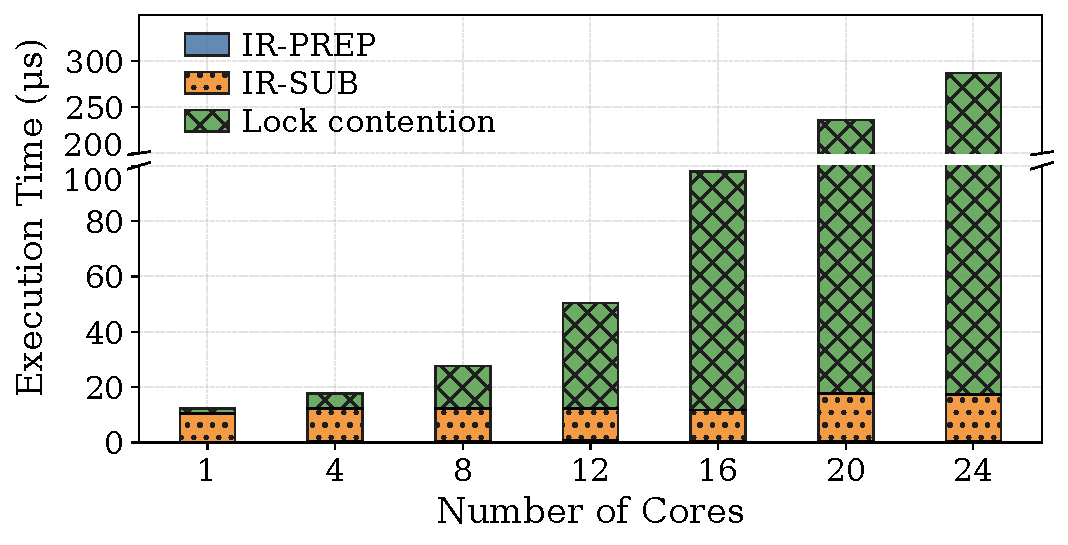
\includegraphics[width=0.7\columnwidth]{figures/siyuan_invalidation_breakdown.pdf}
% \Description{Lock Contention Time Balloons with increasing core count}
\caption{\small {\bf Breakdown of IO memory protection overheads.} IR-PREP contributes minimally, independent of number of cores. For fewer than $8$ cores, IR-SUB cost dominates; for $8$ and more cores, lock contention overheads dominate. Moreover, with increasing number of cores, lock contention time increases superlinearly while the IR-SUB cost remains nearly constant.
}
% \saksham{Linear plot with broken y-axis here.}}
\label{vfree:fig:lock-contention}
\end{figure}

Figure~\ref{vfree:fig:lock-contention} shows the consequence: 
  as the number of vCPUs increases, the time spent waiting 
  to acquire \CodeIn{cache\_lock} grows, 
  while the time for IR-PREP and IR-SUB themselves remains 
  nearly constant. In other words, the actual work per invalidation grows only modestly with scale---the dominant increase is wasted time 
  spent serializing behind other vCPUs.
Each vCPU blocks on its \CodeIn{unmap} call for the duration 
  of this wait, so per-vCPU throughput drops as contention 
  increases.

\if 0
The serialization limits the maximum rate at which the guest can perform \CodeIn{unmap} 
  per unit time (denoted as $R$), independent of the number of concurrent cores performing them: 
  $R < 1/L$ where $L$ is the time to execute the critical section of \CodeIn{cache\_lock}, \textit{i.e.}, the time 
    to execute both IR-PREP and IR-SUB operations. 
The serialization also limits the number of unmap operations 
  needed per unit of transferred network data: if we require an unmap for every $k$ pages transferred on average, 
  the achieved throughput $T < k \times 4KB / L$. For example, for the Tx-host case, 
  we measured $k = 5.5$ ($k>1$ because \CodeIn{map()}/\CodeIn{unmap()} can be performed on 
  a batch of packets in Linux~\cite{Rubin2024FastSafe}). 
  We also measured {$L = 10{\mu}s$}, giving us $T = {\sim}18$Gbps; 
  the observed Tx-host saturation throughput (${\sim}15$Gbps) is within this bound. \rachit{this paragraph is stating the obvious (throughput inversely proportional to lock contention time), brings up unnecessary issues (we never talked about batching in datapath) and is distracting; I suggest removing it.}

% The Serialization especially hurts the performance above because of the large value of $L$. 
Importantly, a majority time out of $L$ (>90\%) is spent on the {\it unavoidable VM exit} 
  required to submit the IR to the IOMMU invalidation queue in the host (see \S\ref{vfree:sec:sec:background-datapath}); 
VM exits typically incur several ${\mu}s$ worth overhead~\cite{vmexit1,vmexit2}. 
While this may have been acceptable with lower I/O speeds in the past, 
  it leads to significantly under-utilized IO bandwidth with 
  current trends of rapidly increasing IO bandwidths. \rachit{if the paper story is about VM exits, this discussion is getting too little real estate.} \rachit{this will benefit significantly from showing the number of VM exits}
\fi 

%  and stagnant VM exit overheads 
%  are leading to larger IO bandwidth underutilized.


% our evaluated workload is a best-case scenario for the optimization, 
%   where the IOVA working set size remains low and thus 
%   most IOVAs used to receive payloads do not require map/unmap operations. 
% However, Rx still needs to perform map/unmap operations for transmitted packets, 
%   such as TCP ACK packets back to the sender. 
% Due to TCP sending aggregated ACKs for multiple packets, the amount of pages transfered per \CodeIn{unmap} (i.e., $k$) 
%   is higher in the Rx case compared to Tx. 
% We measured $k$ to be ${\sim}15\times$ higher, and correspondingly the maximum achievable throughput (${\sim}215$Gbps), 
%   which is still significantly lower than the I/O bandwidth (400Gbps). 
% The maximum measured throughput (145Gbps) lies well within this bound. \rachit{this paragraph could be reduced to 1 line: rx has higher throughput due to optimizations discussed in 2.2 (give them some name) and due to ACK coelescing on the Rx side; note that this is not too important.}

\if 0
\begin{figure}[H]
	\centering
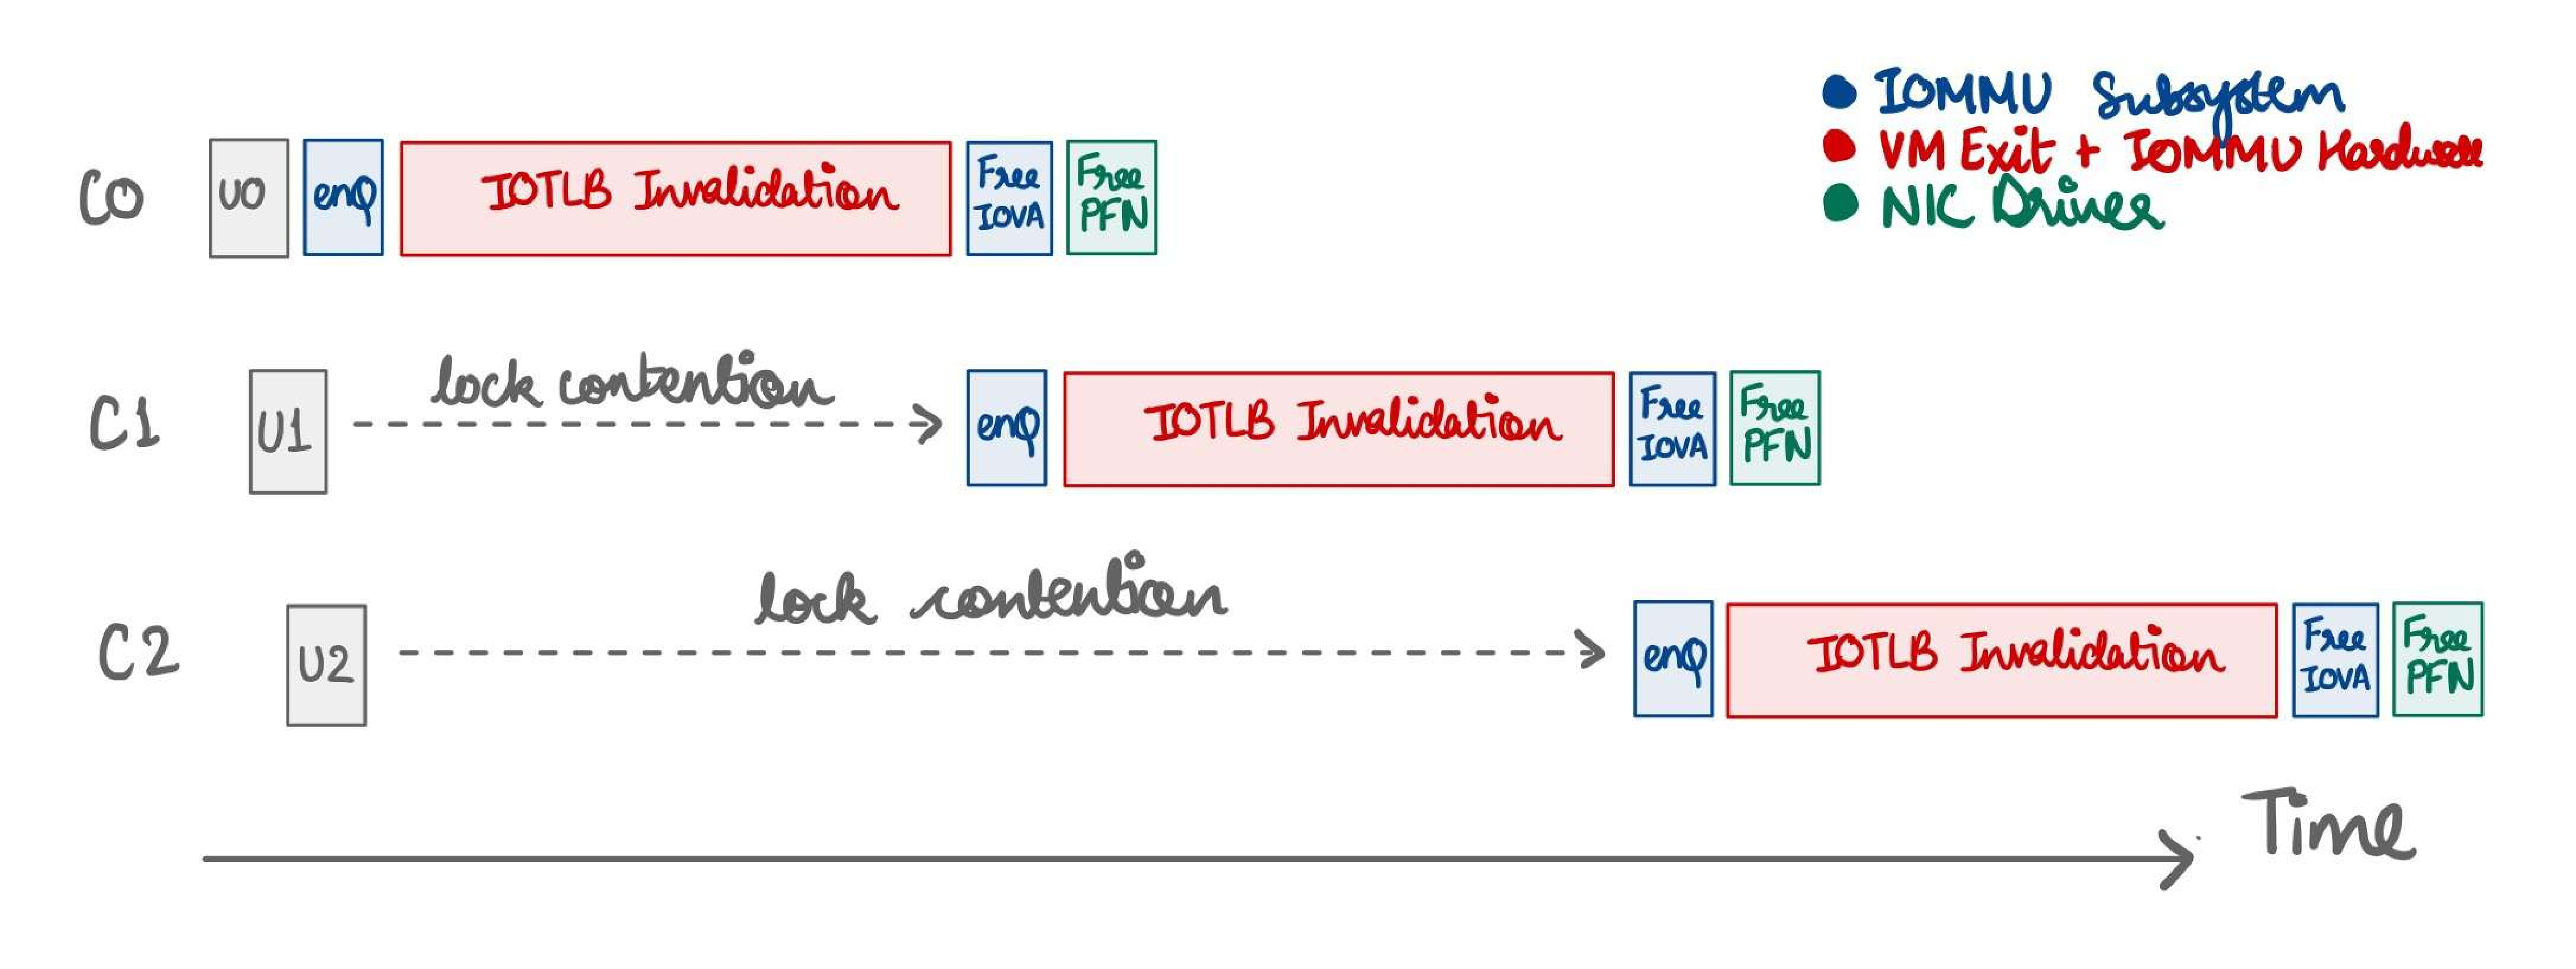
\includegraphics[width=\columnwidth]{figures/hd-default-serialization.pdf}
\Description{Serialization in current strict}
\caption{\saksham{Add pipeline bubbles here because of thread wakeups, leading to lower throughput}}
\label{vfree:fig:current-design-hlt}
\end{figure}
\fi 

\begin{figure}[H]
	\centering
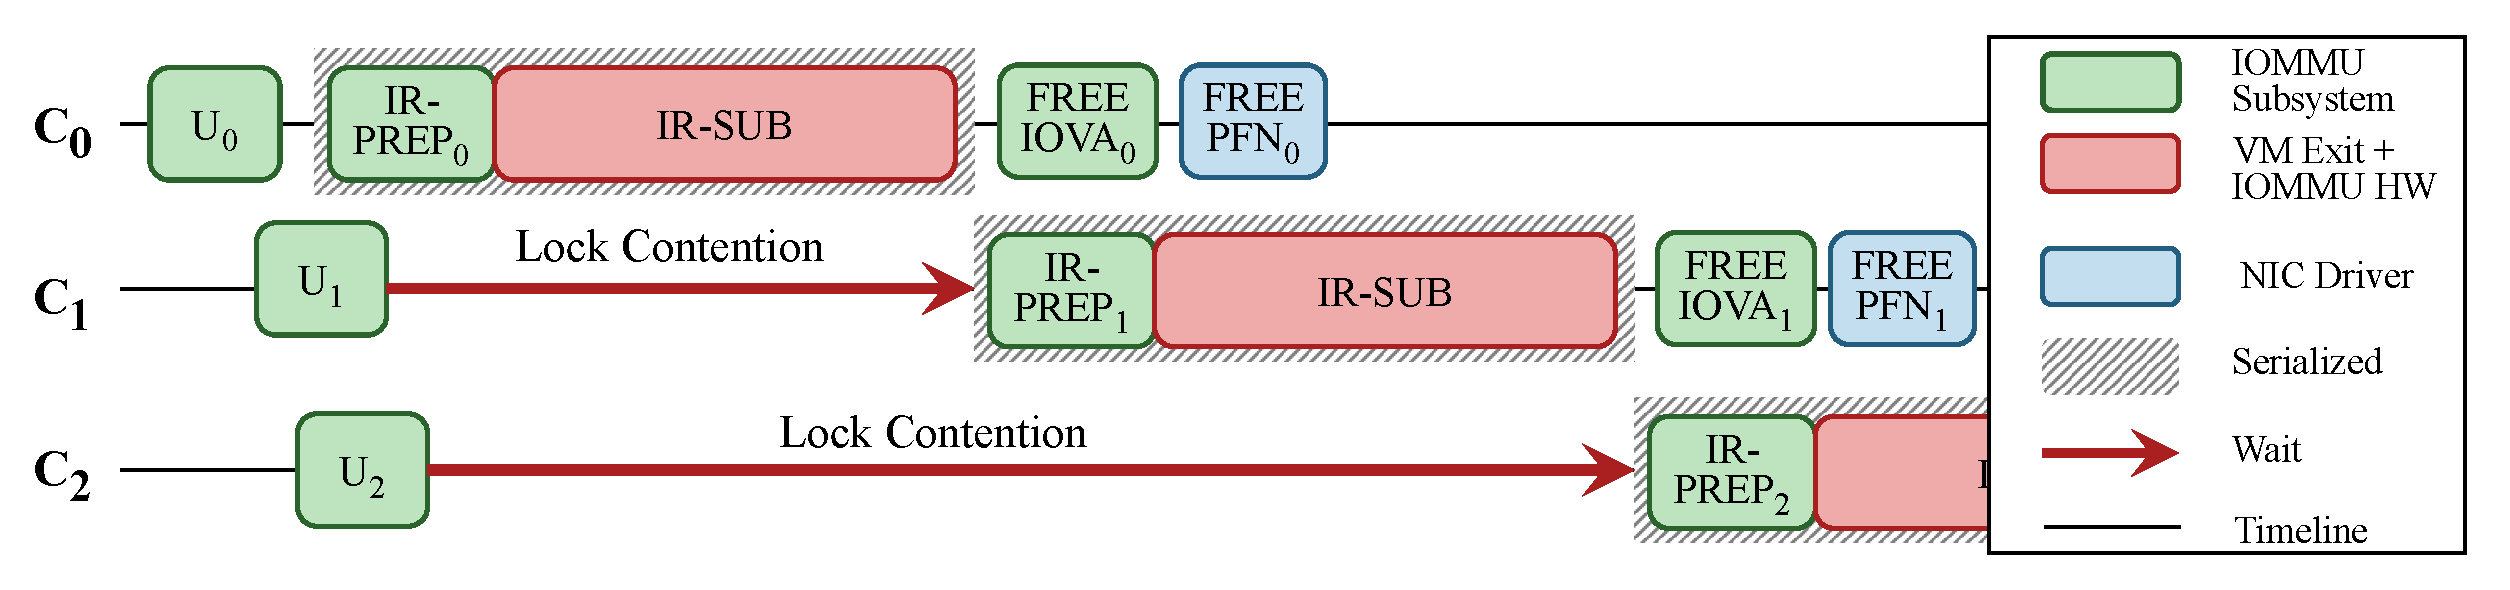
\includegraphics[width=\columnwidth]{figures/strict_serialize_v2_cropped.pdf}
\Description{Serialization in current strict}
\caption{\small {\bf Illustration of strict serialization of each IR-PREP and IR-SUB in existing strict IO memory protection mechanisms across CPU cores ($C_{0,1,2}$).}}
\label{vfree:fig:current-design}
\end{figure}

% \begin{figure}
% 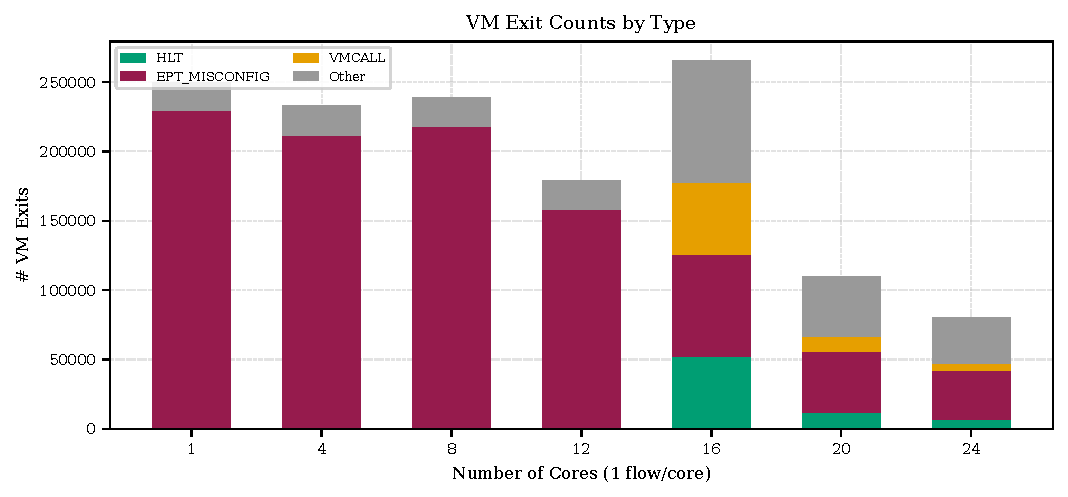
\includegraphics[width=\columnwidth]{figures/vm_exit_counts.pdf}
% \Description{Number of VM exits by exit reason on a single profiled core across increasing core counts. EPT\_MISCONFIG counts decline steadily while PAUSE\_INSTRUCTION, HLT, and VMCALL counts surge between 12 and 16 cores.}
% \caption{VM~exit counts by event type on a single profiled core.
% EPT\_MISCONFIG exits (completed invalidations) decline as contention grows, while PAUSE\_INSTRUCTION and HLT/VMCALL exits surge between 12 and 16~cores}
% \label{vfree:fig:vm-exit-count}
% \end{figure}

% \todo{LESHNA: add pause as separate in vm exit count}

\paragraphb{[Figure~\ref{vfree:fig:lock-contention}] Root cause of throughput reduction at large core counts: % in Figure~\ref{vfree:fig:baseline-iperf}: 
contention-descheduling feedback loop in virtualized environments} We now explain the root causes behind the counter-intuitive observation of throughput reducing with number of cores increasing beyond 12.

% VM exits can happen due to many reasons; Figure~\ref{vfree:fig:vm-exit-time-pct} shows the average time spent on VM~exits on a per \CodeIn{unmap} basis, broken down by events that trigger the VM exit.
% due to all VM exits. 
We observe that two kinds of VM exits dominate. First, VM exits due to MMIO writes to the IOMMU invalidation tail register---``useful work'' of the \CodeIn{unmap} path. Second, VM~exits due to contention-induced vCPU descheduling (triggered by \texttt{HLT} event).
In virtualized environments, an \texttt{HLT} halts a vCPU and triggers a VM~exit that causes KVM to deschedule the vCPU till an interrupt or wake event arrives.

We observe that, at low core counts, nearly all per-\CodeIn{unmap} VM~exit time (${\sim}$94\%) is spent in handling writes to the MMIO invalidation queue tail register 
% in VM exits  due to the \texttt{EPT\_MISCONFIG} event 
and the total per-\CodeIn{unmap} exit cost is ${\sim}$11--18\,$\mu$s (IR-SUB cost in Figure~\ref{vfree:fig:lock-contention}).
At 16~cores and above, contention-induced descheduling consumes
  % \texttt{HLT}-induced VM~exits consume
 {93--97\%} of per-\CodeIn{unmap} exit time, inflating the total cost to 141\,$\mu$s at 16~cores and \textit{514\,$\mu$s} at 24~cores---a $46\times$ increase over the low-contention baseline.
 The reason is as follows.

% \begin{figure}
% 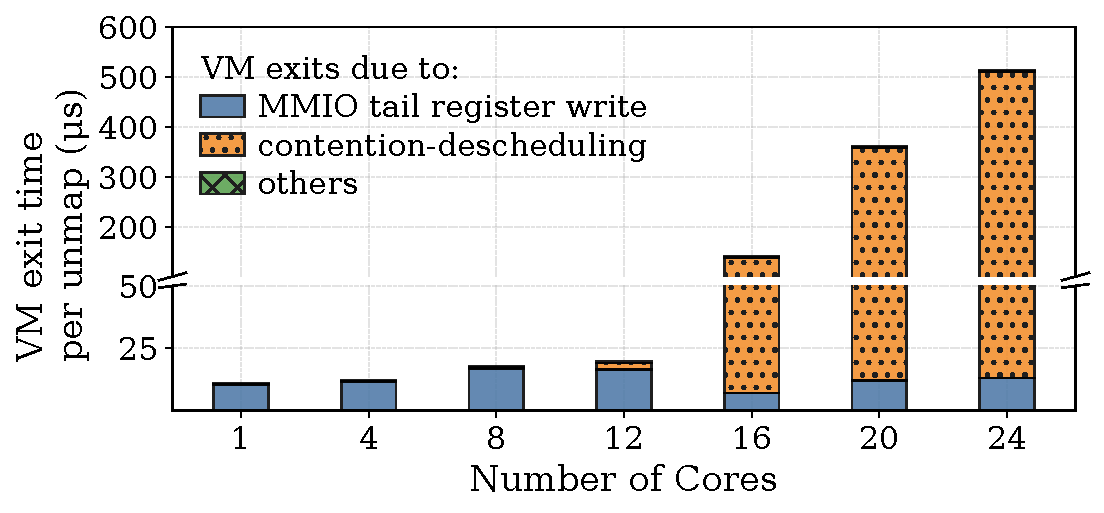
\includegraphics[width=\columnwidth]{figures/vm_exit_time_per_unmap.pdf}
% % \Description{Average VM exit time per unmap operation speant on HLT and EPT\_MISCONFIG across increasing core counts. At low core counts EPT\_MISCONFIG dominates; beyond 16 cores HLT dominates.}
% \vspace{-15pt}
% \caption{\small {\bf Breakdown of average VM~exit time per \CodeIn{unmap} operation due to various events that trigger VM exits.} At low core counts, nearly all per-\CodeIn{unmap} VM~exit time is spent in handling writes to the MMIO invalidation queue tail register; at 16~cores and above, contention-induced descheduling consumes contributes to most of the per-\CodeIn{unmap} exit time. \rachit{make a note on why this figure y-axis has scale higher than figure 5 y-axis scale (why is average HLT time higher than average execution time---the normalization factor for averages uses different number of cores in the two}}
% \vspace{-10pt}
% \label{vfree:fig:vm-exit-time-pct}
% \end{figure}


\para{Contention-descheduling feedback loop.}
The transition from useful work to idle waiting follows a three-stage cascade process visible in the VM~exit data:

\begin{enumerate}
\item {\it Spinning.}
  As vCPU count grows, more vCPUs contend for \CodeIn{cache\_lock}.
  Waiters spin in tight \CodeIn{PAUSE} loops, waiting for the lock holder to complete its invalidation.
  We find that, from 12 to 16 cores,
  \CodeIn{PAUSE}-related VM exits
  increase by {$60\times$}, triggered by the processor's Pause-Loop Exiting (PLE) mechanism,
  which detects sustained spinning and traps to the
  hypervisor once a threshold is exceeded~\cite{Shan2017apples}.
\item \textit{Descheduling.}
  Once a vCPU has exceeded its spin budget,
\if 0
  \footnote{Increasing the 
  PLE spin budget (\textit{i.e.}, \texttt{PLE\_window}) 
  delays the onset of this cascade to higher core counts 
  but does not prevent it: the fundamental throughput ceiling 
  is set by the serialized invalidation path, not by the 
  spin threshold.
  Kashyap et al.~\cite{Kashyap2016oppspinlocks} observe that 
  the collapse simply shifts rightward with a larger budget, 
  and Shan et al.~\cite{Shan2017apples} show that 
  no static threshold is optimal across workloads.},
\fi
  an \CodeIn{HLT} event is triggered, which leads to another VM exit that causes
  the host (KVM) deschedules the vCPU.
  We confirmed that these \CodeIn{HLT}-related VM exits are lock-induced halts, and not due to idle vCPUs. 
  % (the so-called \CodeIn{VMCALL}-induced wakeups~\cite{KVM_KICK_VM_CALL}
  % track almost exactly with \CodeIn{HLT}-related VM exits). 
  The same phenomenon is observed for general kernel spinlocks:
  at a high contention level, most vCPUs
  simultaneously fail their optimistic spin
  and trap to the hypervisor~\cite{Kashyap2016oppspinlocks}.

  
  
  % jump from 588 to 52,265
  % between 12 and 16 cores,
  % tracking \CodeIn{VMCALL} almost exactly
  % (469 to 51,648), confirming these are lock-induced halts, not idle vCPUs.


\item \textit{Expensive wakeup.}
  When the lock holder finishes and
  releases \CodeIn{cache\_lock}, the next waiter must be
  woken via an IPI.
This wakeup path, which is cheap on bare metal (${\sim}$8\,$\mu$s),
  is an expensive event in virtualized environments,
  known as the \emph{Blocked-Waiter Wakeup} (BWW) problem~\cite{Ding2014gleaner}:
  the IPI triggers a VM~exit on the vCPU that triggers the wakeup event, invokes the KVM scheduler,
  and requires a VM~entry to reschedule the target vCPU. The latency for the wakeup path is included in the \CodeIn{HLT} duration.
%  with a penalty factor of 
%  4.6--6.2$\times$ even with dedicated CPU pinning
% BWW arises whenever blocking synchronization 
%  executes in a virtualized environment, 
%  causing increased execution times and reduced 
%  throughput~\cite{Ding2014gleaner}.
In our measurements, average \texttt{HLT} duration per unmap
  grows from $2.5\mu$s at $12$~cores to 131\,$\mu$s at 16~cores to $346\mu$s at 20~cores to $498\mu$s at 24~cores, far exceeding a single BWW event because the cost compounds:
  as more vCPUs are descheduled simultaneously, 
  each must wait longer to be rescheduled,
  and the vCPU responsible for sending wakeup IPIs
  may be contending for the same lock.
% \schaic{
% Do we want the average per call HLT (what we have in the text) or HLT time per unmap (Fig6).}
% During this wakeup window, no core holds the lock.
%  creating idle bubbles on the hardware invalidation queue.
\end{enumerate}
% The three stages form a \emph{positive feedback loop}:
%  contention causes descheduling,
%  descheduling inflates wakeup latency,
%  longer wakeups leave the lock unheld 
%  (introducing pipeline bubbles on the invalidation queue),
%  which increases the effective time between
%  consecutive invalidation completions as seen by
%  all waiting vCPUs---causing more of them to exceed 
%  their spin budgets and be descheduled.
This feedback loop results in {\it super-linear} increase in \CodeIn{HLT}-related VM exit time:
  for the core on which we profile, ${\sim}$157K invalidations are completed for 12~cores
  but only ${\sim}$35K invalidations are completed for 24~cores, a $4.5\times$ reduction with merely $2\times$ increase in number of cores. %---while
%   the average cost of each individual invalidation grows only
%   $1.7\times$ (8.3\,$\mu$s to 14.3\,$\mu$s).
% The remaining ${\sim}3.8\times$ gap
%   is entirely time spent descheduled.

This feedback loop is specific to virtualized environments.
On bare metal, a spinning thread remains on its physical
  core and resumes immediately when the lock is released;
  the virtualization layer converts what would be a brief
  spin-wait into a cascade of VM~exits whose cost compounds
  with every additional contending vCPU.
The individual pathologies---PLE-triggered 
  descheduling~\cite{Shan2017apples}, 
  mass halt under contention~\cite{Kashyap2016oppspinlocks}, 
  and BWW~\cite{Ding2014gleaner, Kashyap2018ecs}---are well studied
  for general kernel spinlocks,
  but the IOMMU invalidation path is a uniquely severe instance:
  the serialized hardware queue is a fixed point
  on every packet's \CodeIn{unmap} that cannot be
  parallelized or avoided.

% \rachit{It would also be nice to show the number of VM exits in Figure~\ref{vfree:fig:vm-exit-time-pct} to further support the evidence.}

% \rachit{if we increased the spin budget, would this phenomenon reduce or even go away for large spin budgets? could we demonstrate that? It would really nail down the problem.} 
% \leshna{added a footnote we can keep if important}
 
